\documentclass[12pt,a4paper,sans, oneside]{book}
\usepackage[top=2cm, bottom=2cm, left=2cm, right=2cm]{geometry} % Reduce document margins

\usepackage{titlesec}
\titleformat{\chapter}[hang]{\normalfont\Large\bfseries}{\thechapter:}{1em}{}
\titleformat{\section}[hang]{\normalfont\large\bfseries}{\thesection}{1em}{}
\titleformat{\subsection}[hang]{\normalfont\large\bfseries\itshape}{\thesubsection}{1em}{}
\titleformat{\subsubsection}[hang]{\normalfont\normalsize\bfseries\itshape}{\thesubsubsection}{1em}{}

% Table of contents formatting
\setcounter{tocdepth}{0}

% numbering shown down to sub-sub-section

\setcounter{secnumdepth}{3}
% Section formatting
\renewcommand\thechapter{\Alph{chapter}}
\renewcommand\thesection{\thechapter.\arabic{section}}
\renewcommand\thesubsection{\alph{subsection})}
\renewcommand\thesubsubsection{\roman{subsubsection}.}
\titlespacing\chapter{0em}{-2em}{0em}
\titlespacing\section{0em}{2em}{0em}
\titlespacing\subsection{0em}{2em}{0em}
\titlespacing\subsubsection{0em}{2em}{0em}

\usepackage[utf8]{inputenc}
\usepackage{fontawesome5}
\usepackage{orcidlink}
\usepackage{fontawesome5}
\usepackage{academicons}

% For subfloat
\usepackage{subfig}
\usepackage{graphicx}

% Foreground & background color management
\usepackage{xcolor}

% Insertable PDFs
\usepackage{pdfpages}

% quotes
\usepackage{csquotes}

% Hyperlinks and urls
\usepackage{hyperref}
\hypersetup{
	colorlinks=true,
	linkcolor=blue!75,
	filecolor=red!75!green!50!blue,
	urlcolor=red!75,
	pdftitle={G. Stark - Academic Qualifications Portfolio},
	pdfpagemode=FullScreen,
}

\usepackage{url}

% DOI
\usepackage{doi}

% Scientific SI units
\usepackage{siunitx}
\usepackage{hepnames}

% Multi-column & multi-row tables
\usepackage{multicol}
\usepackage{multirow}

% Formatting lists
\usepackage{enumitem}

% Fancy headers package
\usepackage{fancyhdr}
\usepackage[font={small}]{caption}
\usepackage[hang,flushmargin]{footmisc}
%\linespread{1.1}
\linespread{1}
\pagestyle{fancy}
\fancyhead{}
\fancyhf{}
\fancyhead[C]{Academic qualifications portfolio for Faculty of Science, Lund University}
%\fancyfoot[L]{Research activity}
\fancyfoot[L]{Dr. G. Stark \faIcon{deaf} $\cdot$ Lunds Universitet $\cdot$ Senior Lecturer PA2024/647\\[-0.2em]{\fontsize{10}{0}\mdseries\upshape Pronouns: point/he/him}}
\rfoot{\thepage}

\usepackage{cleveref}

% https://tex.stackexchange.com/a/117334
% use fancyhdr on chapter pages
\usepackage{etoolbox}
\patchcmd{\chapter}{\thispagestyle{plain}}{\thispagestyle{fancy}}{}{}

% Create a custom command for formatting my project descriptions
% Project name, time period, collaboration, location
\newcommand{\ProjectSummary}[5]{\noindent\textbf{#1} \hfill #2 \\ \textit{#3} \hfill \textit{#4} \\ \textit{Collaborating institutions:} #5 }

\newcommand{\Activity}[4]{\noindent\textbf{#1} \hfill #2 \\ \textit{#3} \hfill \textit{#4} }

% Custom command for recommenders
\newcommand{\Recommender}[3]{\noindent\textbf{#1}, \textit{#2}, \faIcon{envelope}~\href{mailto:#3}{#3} }

% Custom command for publications
\newcommand{\Publication}[6]{\noindent\colorbox{#1}{\textcolor{#2}{\textbf{#3}}}~#5\hfill\doi{#4} \\ #6}

% For numbering publications
\newcommand{\PubCite}[3]{\colorbox{#1}{\textcolor{#2}{\textbf{#3}}}}

% Footnotes
\renewcommand{\thefootnote}{\alph{footnote}}

% Drafting assistance
%\usepackage[doublespacing]{setspace}
%\usepackage{lineno}
%\linenumbers

%%::: Custom commands
% "None yet" and "none" tags for section headers
\newcommand{\noneyet}{\normalsize{\textit{-- none yet}}}
\newcommand{\none}{\normalsize{\textit{-- none}}}

\newcommand{\phonesymbol}{\faIcon{phone}\ }
\newcommand{\emailsymbol}{\faIcon{envelope}\ }
\newcommand{\addresssymbol}{\faIcon{location-arrow}\ }
\newcommand{\mobilesymbol}{\faIcon{mobile}\ }
\newcommand{\homepagesymbol}{\faIcon{link}\ }

\usepackage[backend=biber,sorting=none]{biblatex}
\addbibresource{bib/main.bib}

\title{\Huge Academic qualifications portfolio for Faculty of Science, Lund University}
\author{\large Dr. Giordon H. Stark\ \faIcon{deaf}\ {\small\color{gray}(pronouns: point/he/him)}\\[1em]\faIcon{university} SCIPP\thanks{Santa Cruz Institute for Particle Physics}, UC Santa Cruz, United States}
\date{}


% DOCUMENT ITSELF
\begin{document}
\addtocontents{toc}{\protect\setcounter{tocdepth}{-1}}
\setcounter{chapter}{8}
\chapter{All attachments and certificates}
\, \\
\addtocontents{toc}{\protect\setcounter{tocdepth}{2}}

\begingroup
\let\clearpage\relax
\tableofcontents*
\endgroup

\clearpage

\setcounter{chapter}{1}
\chapter{Curriculum vitae}
\begin{figure}[h!]
	\centering
	\caption{\textbf{California Institute of Technology, B.S. in Physics, 2012.}}
	
\includegraphics[width=0.9\textwidth]{attachments/B-CV/BS}
\end{figure}

\begin{figure}[h!]
	\centering
	\caption{\textbf{University of Chicago, Ph.D. in Physics, 2018.}}
	
\includegraphics[width=0.9\textwidth]{attachments/B-CV/PhD}
\end{figure}

\begin{figure}[h!]
	\centering
	\caption{\textbf{CERN}: Fellow contract}
	
\includegraphics[width=0.9\textwidth]{attachments/B-CV/cernFellowContract.pdf}
\end{figure}

\setcounter{chapter}{3}
\chapter{Research qualifications portfolio}

\begin{figure}[h!]
	\centering
	\caption{\textbf{DOE-SCGSR}: Letter of Appointment}
	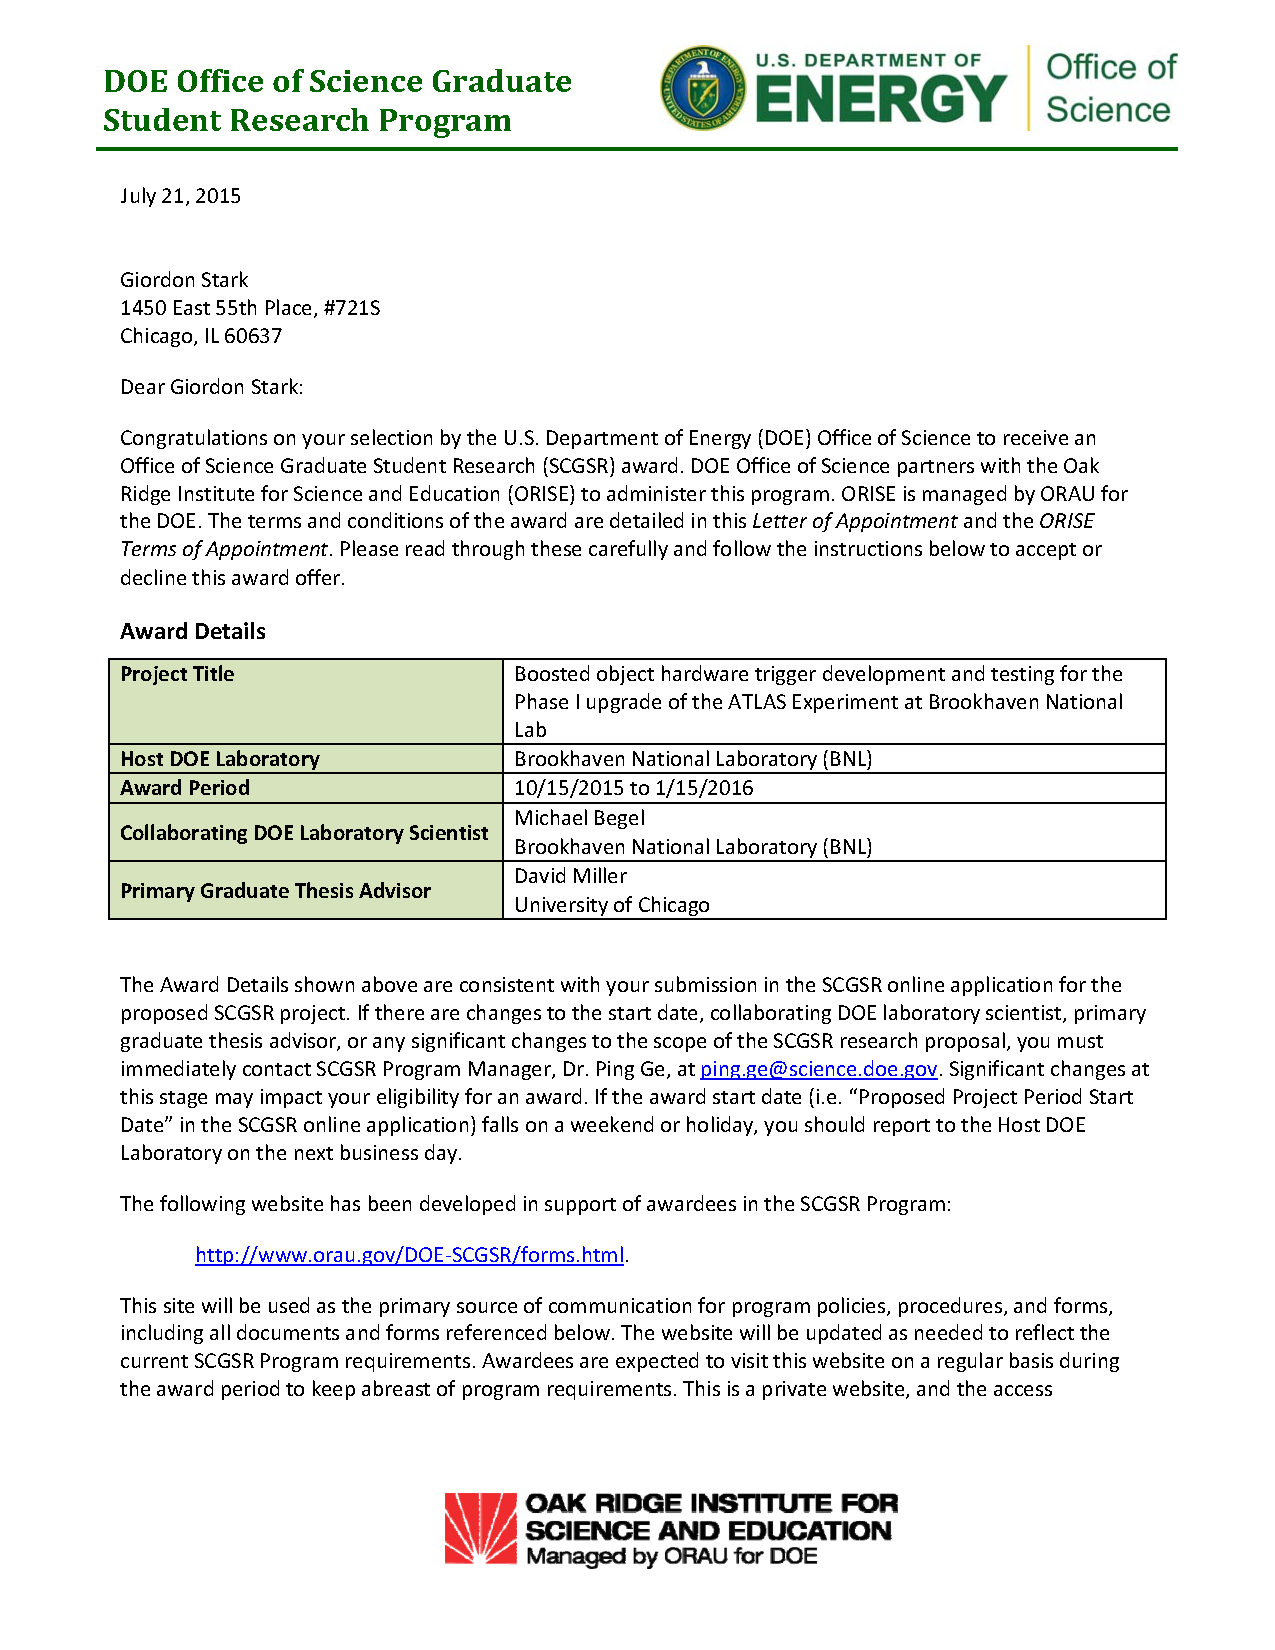
\includegraphics[width=0.9\textwidth]{attachments/D-research/DOE-SCGSR-Letter_of_Appointment}
\end{figure}

\begin{figure}[h!]
	\centering
	\caption{\textbf{Nathan Sugarman Award}: Excellence in Graduate Student Research. \enquote{For his technical contributions and creative insights in the design and prototyping of a new high-speed electronics trigger system for lorentz-boosted massive particles for the ATLAS Experiment.} The Sugarman Award recognizes one of Nathan's highest priorities: encouraging young scientists. It was both the interdisciplinary research at the Institute, and the education of students, to which he devoted his scholarly life.}
	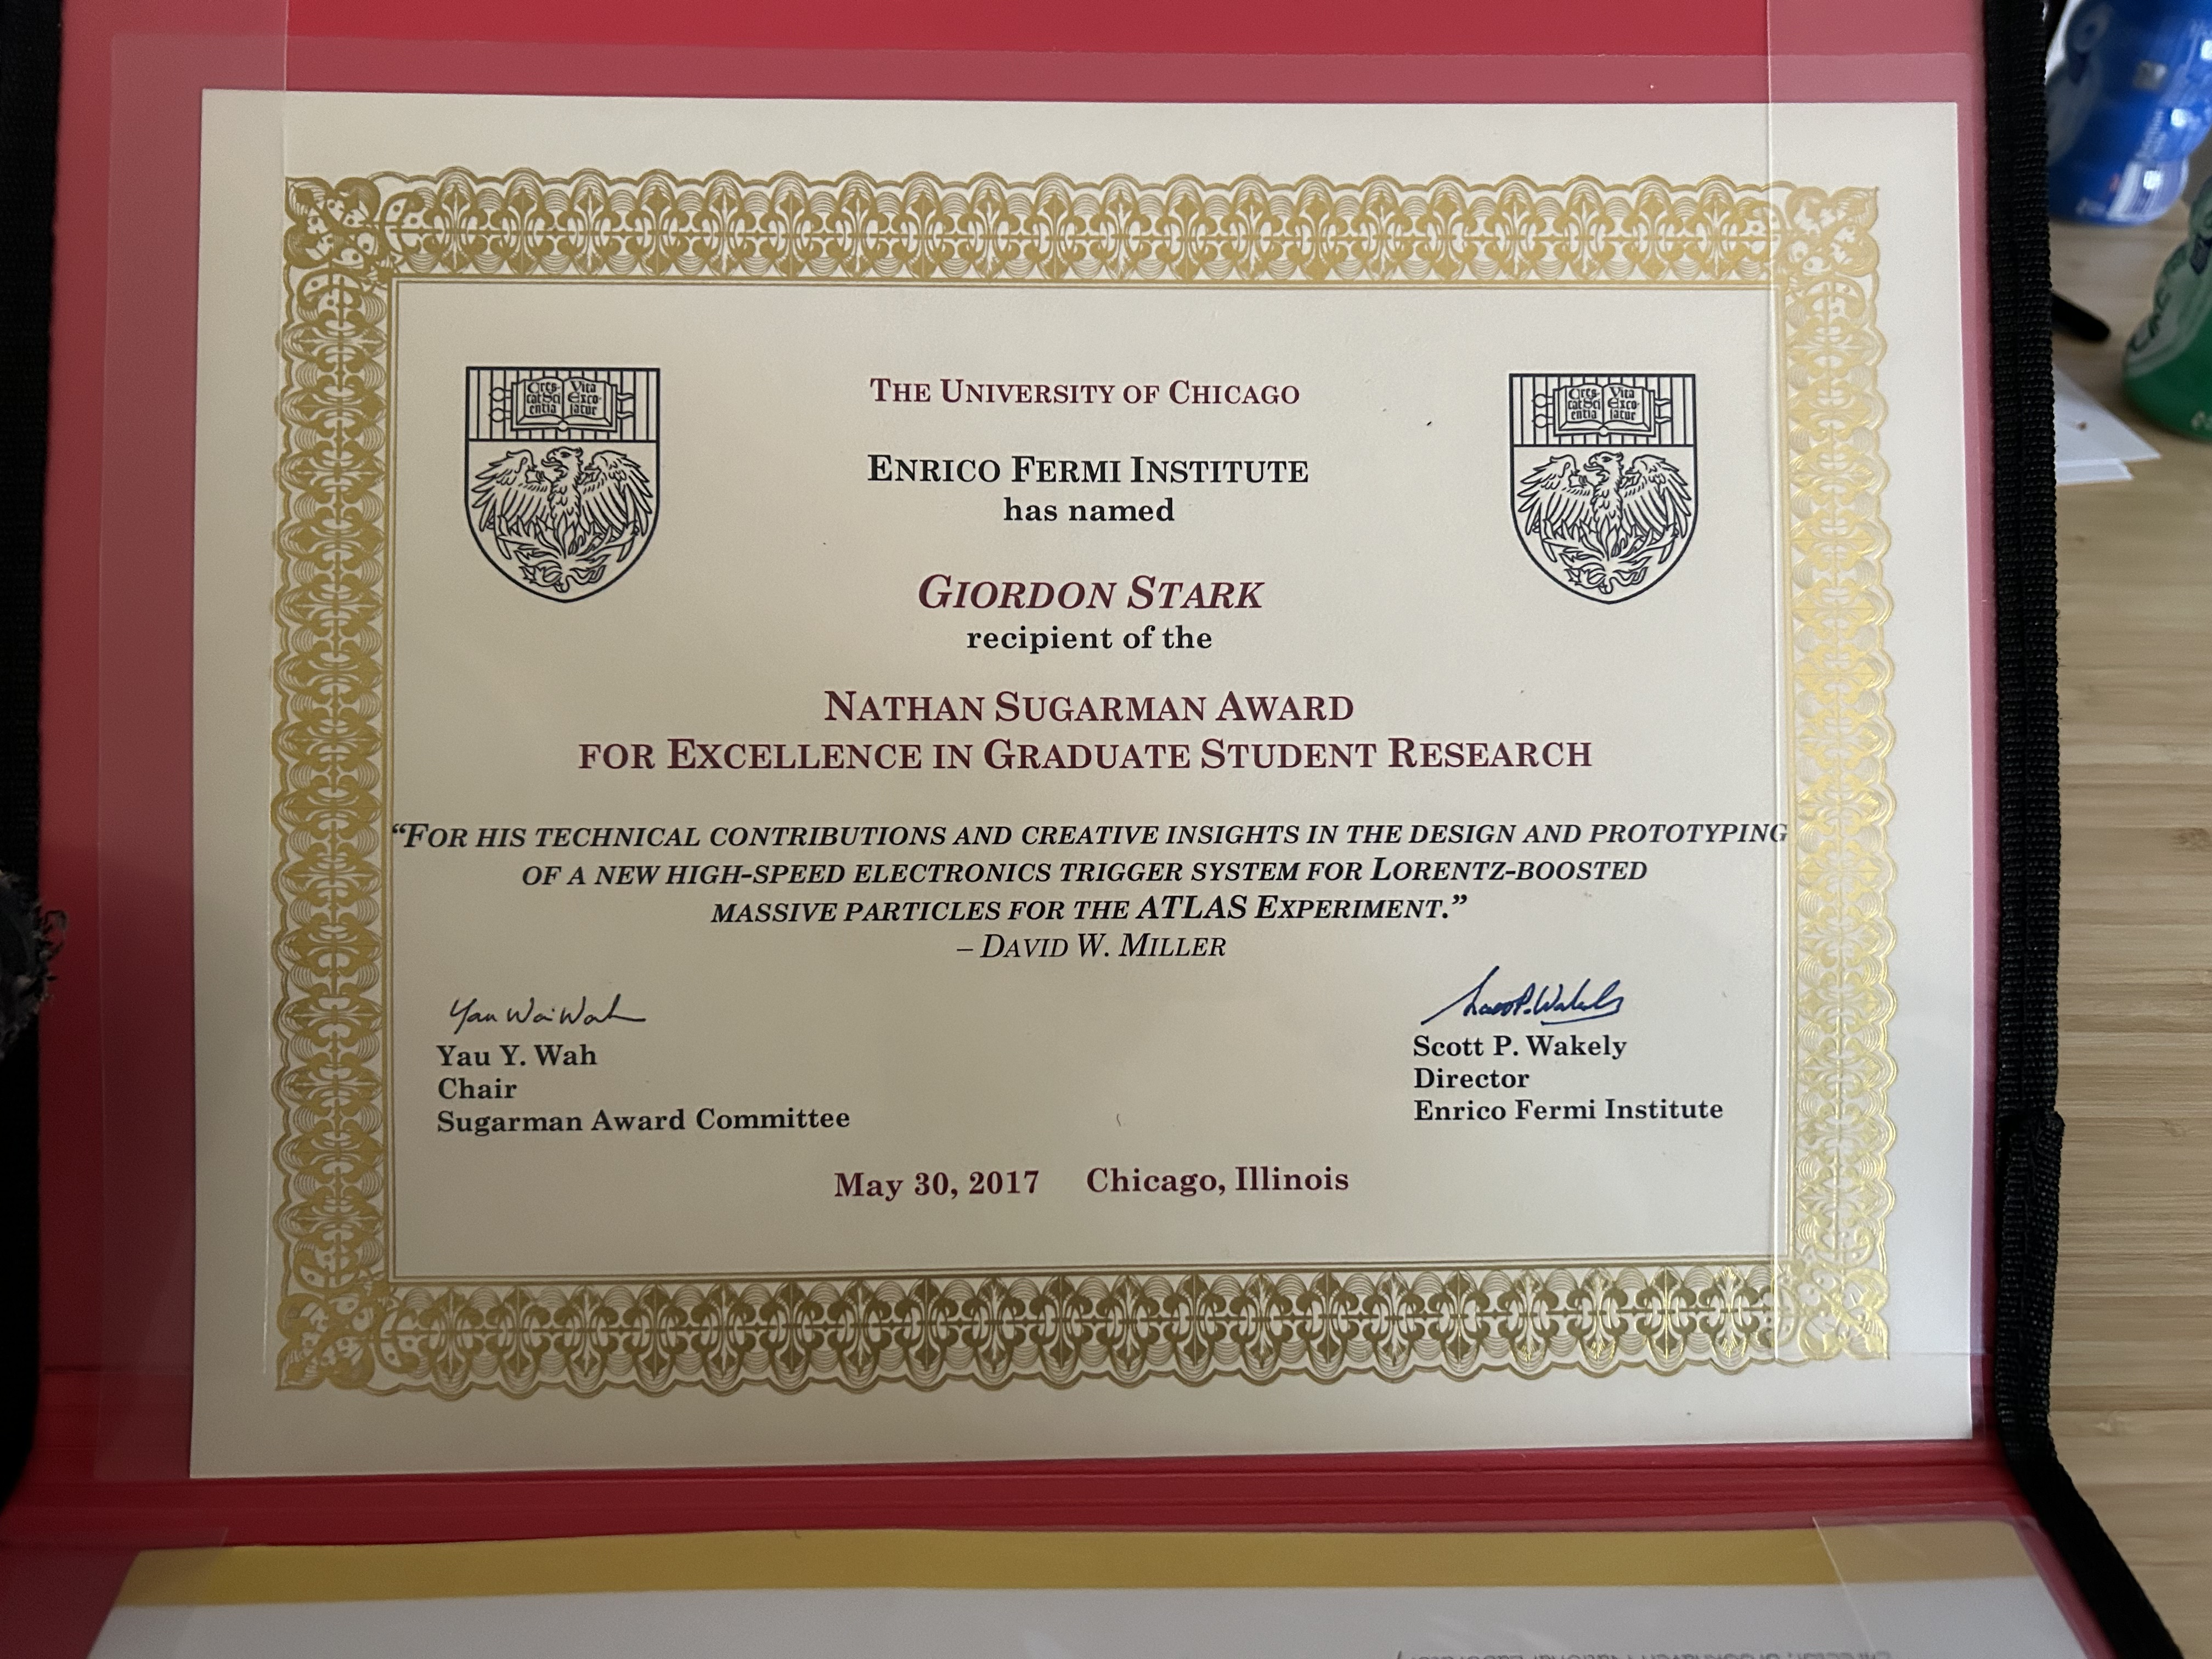
\includegraphics[width=0.9\textwidth]{attachments/D-research/nathanSugarman}
\end{figure}

\begin{figure}[h!]
	\centering
	\caption{\textbf{Springer Thesis Award}: an email from the editor. The series \enquote{Springer Theses} brings together a selection of the very best Ph.D. theses from around the world and across the physical sciences. Nominated and endorsed by two recognized specialists, each published volume has been selected for its scientific excellence and the high impact of its contents for the pertinent field of research.}
	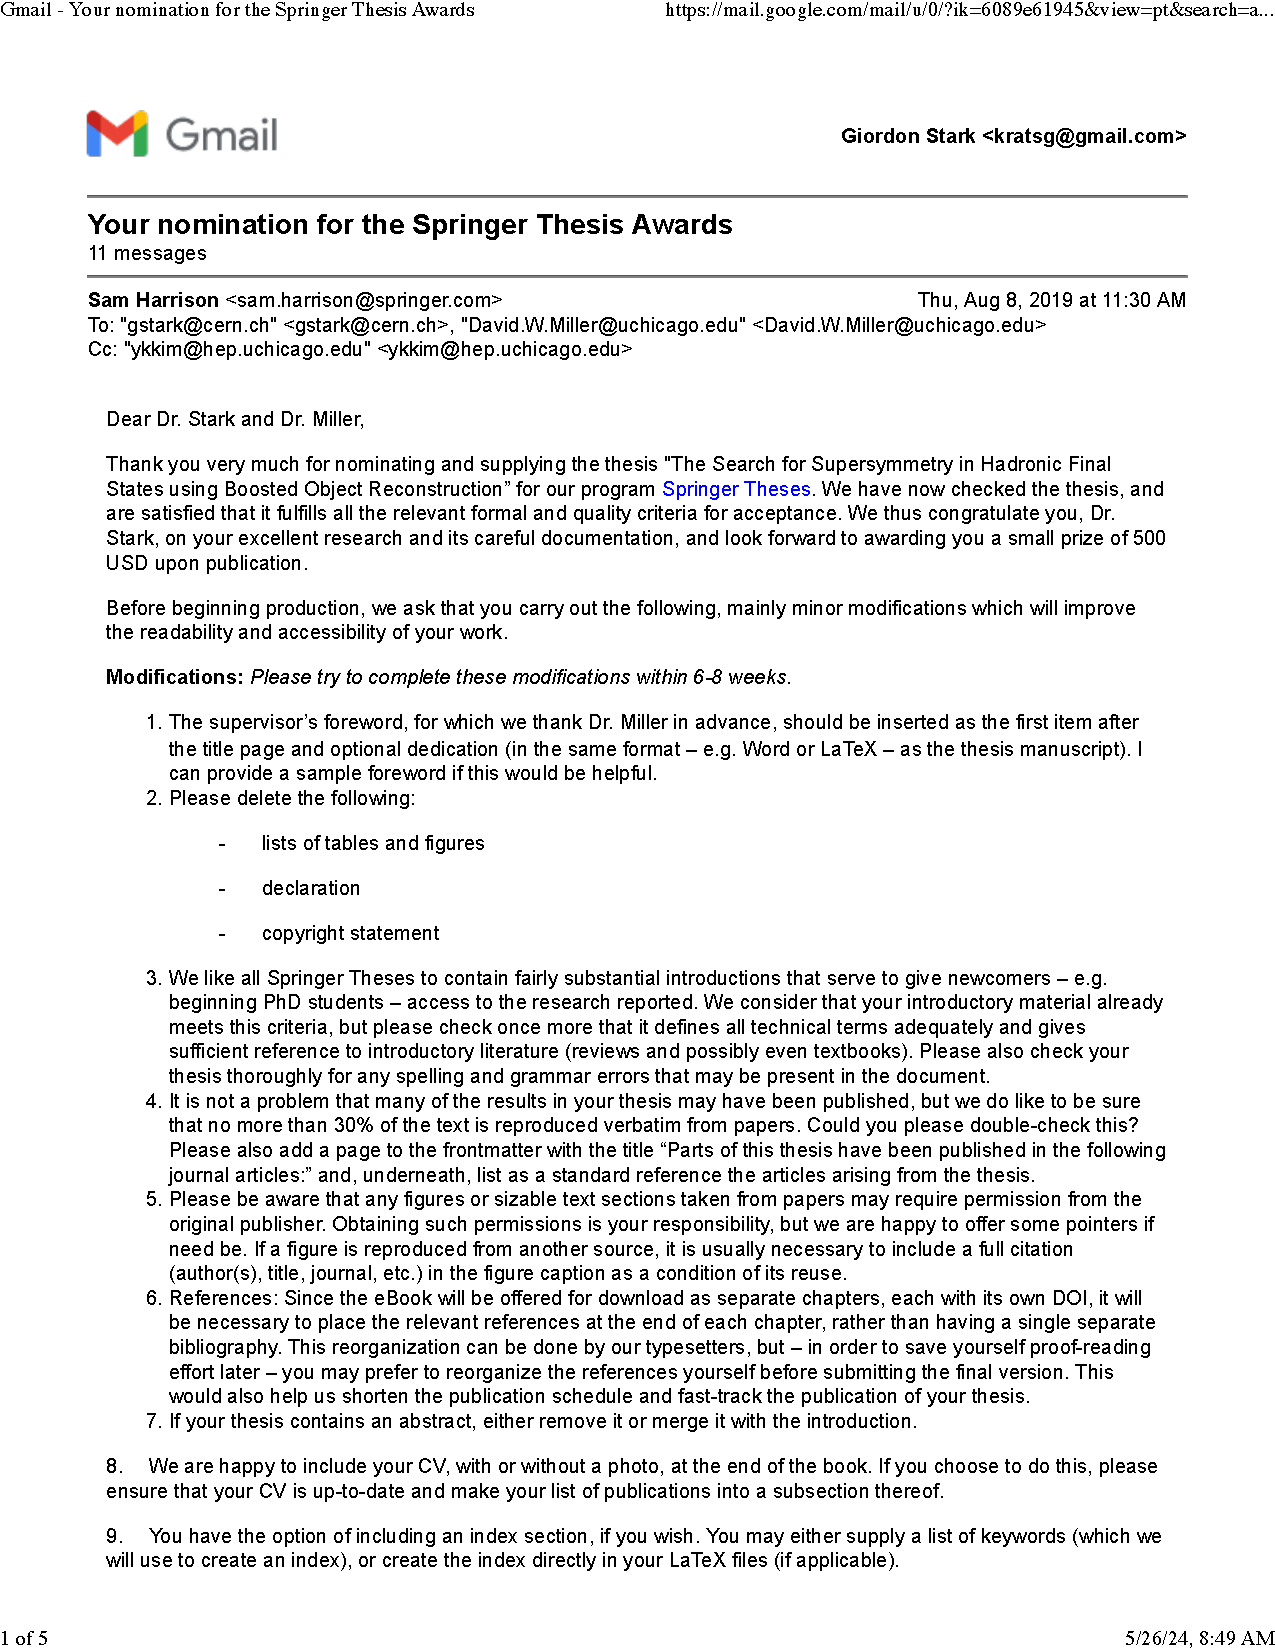
\includegraphics[width=0.9\textwidth]{attachments/D-research/springerThesisAward}
\end{figure}

\begin{figure}[h!]
	\centering
	\caption{\textbf{UCSC Outstanding Postdoctoral Fellow Award}: an email from the Graduate Division Outstanding Postdoctoral Fellow selection committee.}
	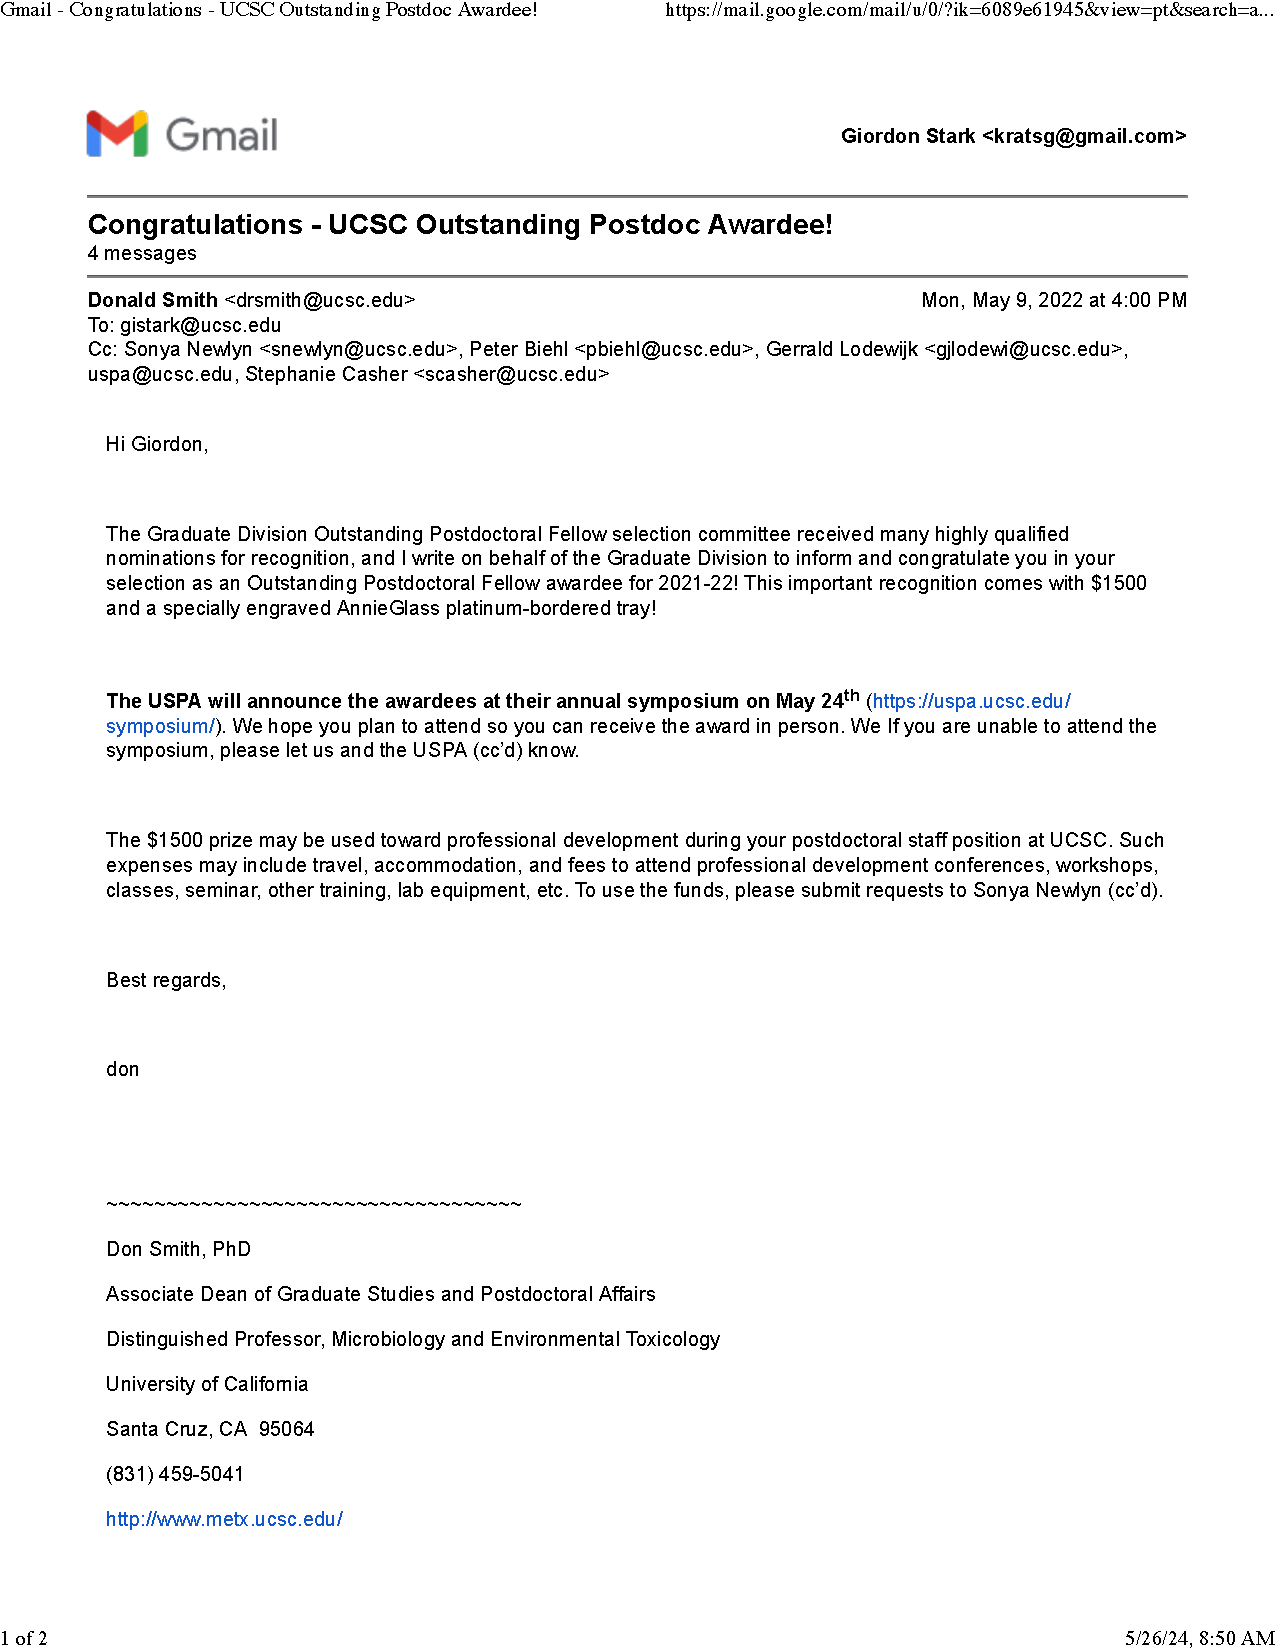
\includegraphics[width=0.9\textwidth]{attachments/D-research/ucscOutstandingPostdocAward}
\end{figure}

\begin{figure}[h!]
	\centering
	\caption{\textbf{US-ATLAS Outstanding Graduate Student Award}: \enquote{In recognition of your exceptionally broad and noteworthy contributions to the ATLAS experiment. In particular, we recognize your critical contributions to the electronics design and prototyping for a new high-speed trigger electronics system for the Phase 1 upgrade, software development, leadership in the creation of a new method to search for Supersymmetry, and software education.}}
	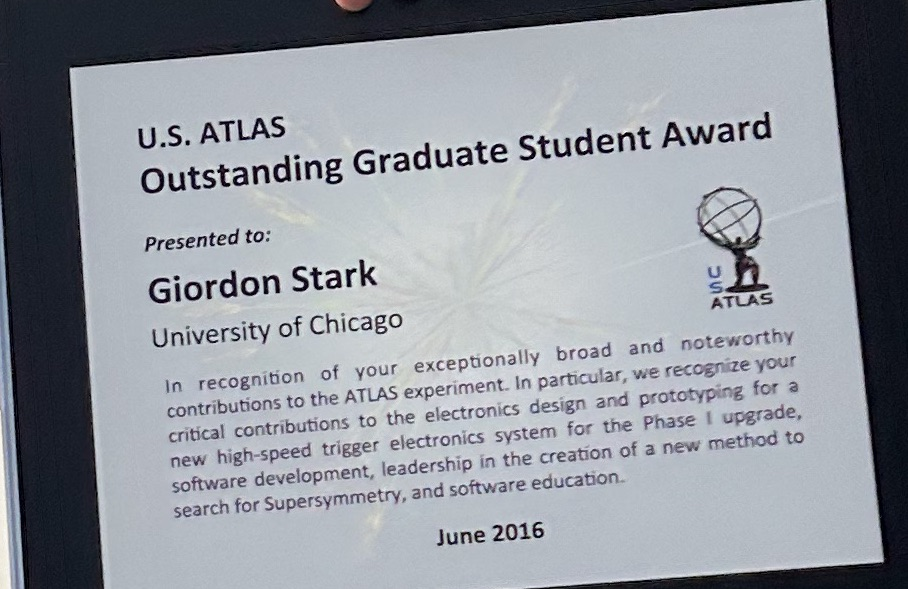
\includegraphics[width=0.9\textwidth]{attachments/D-research/usatlasOutstandingGradStudent}
\end{figure}

\begin{figure}[h!]
	\centering
	\caption{\textbf{Young Researchers' Symposium Award}: outstanding poster presentation.}
	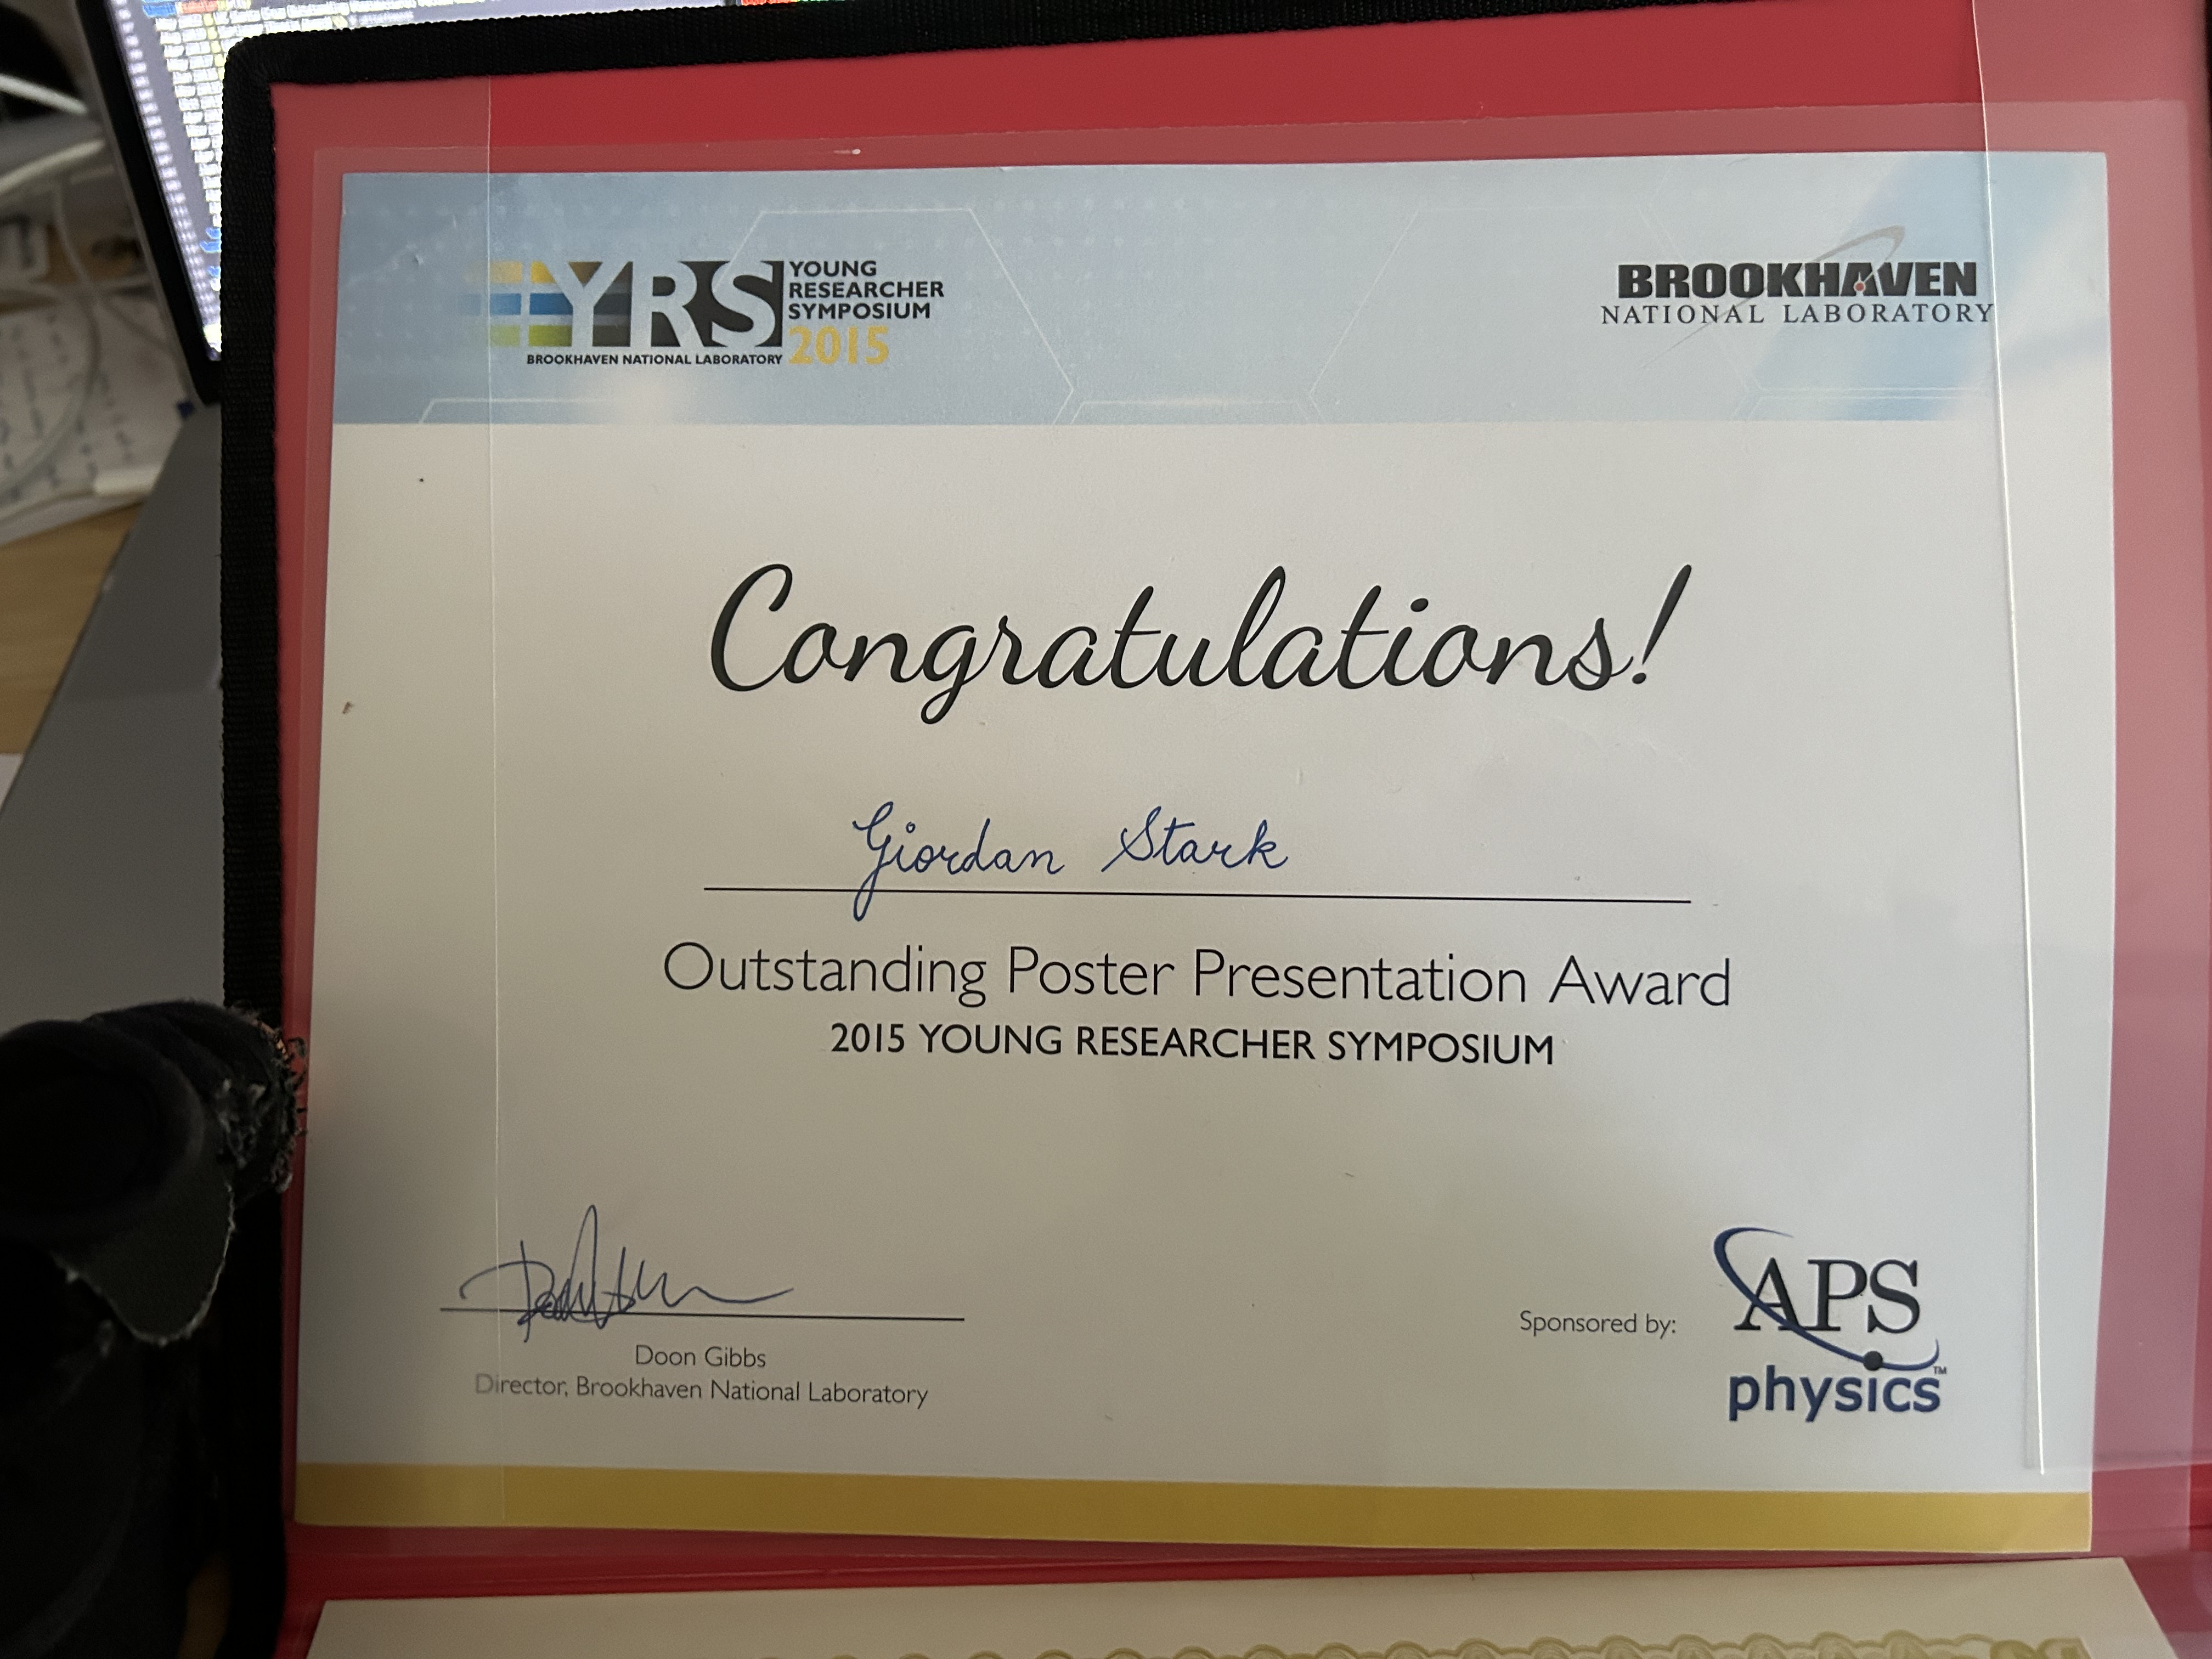
\includegraphics[width=0.9\textwidth]{attachments/D-research/YRS2015}
\end{figure}

\begin{figure}[h!]
	\centering
	\caption{\textbf{US LHC Users' Association Award}: outstanding lightning talk. This is an email from an organizer for the \enquote{DC Policy Trip}. The awardees are invitated to participate in an outreach / policy formation trip to Washington D.C. to meet with members of Senate and Congress to advocate for the messaging in the APS P5 2013 report.}
	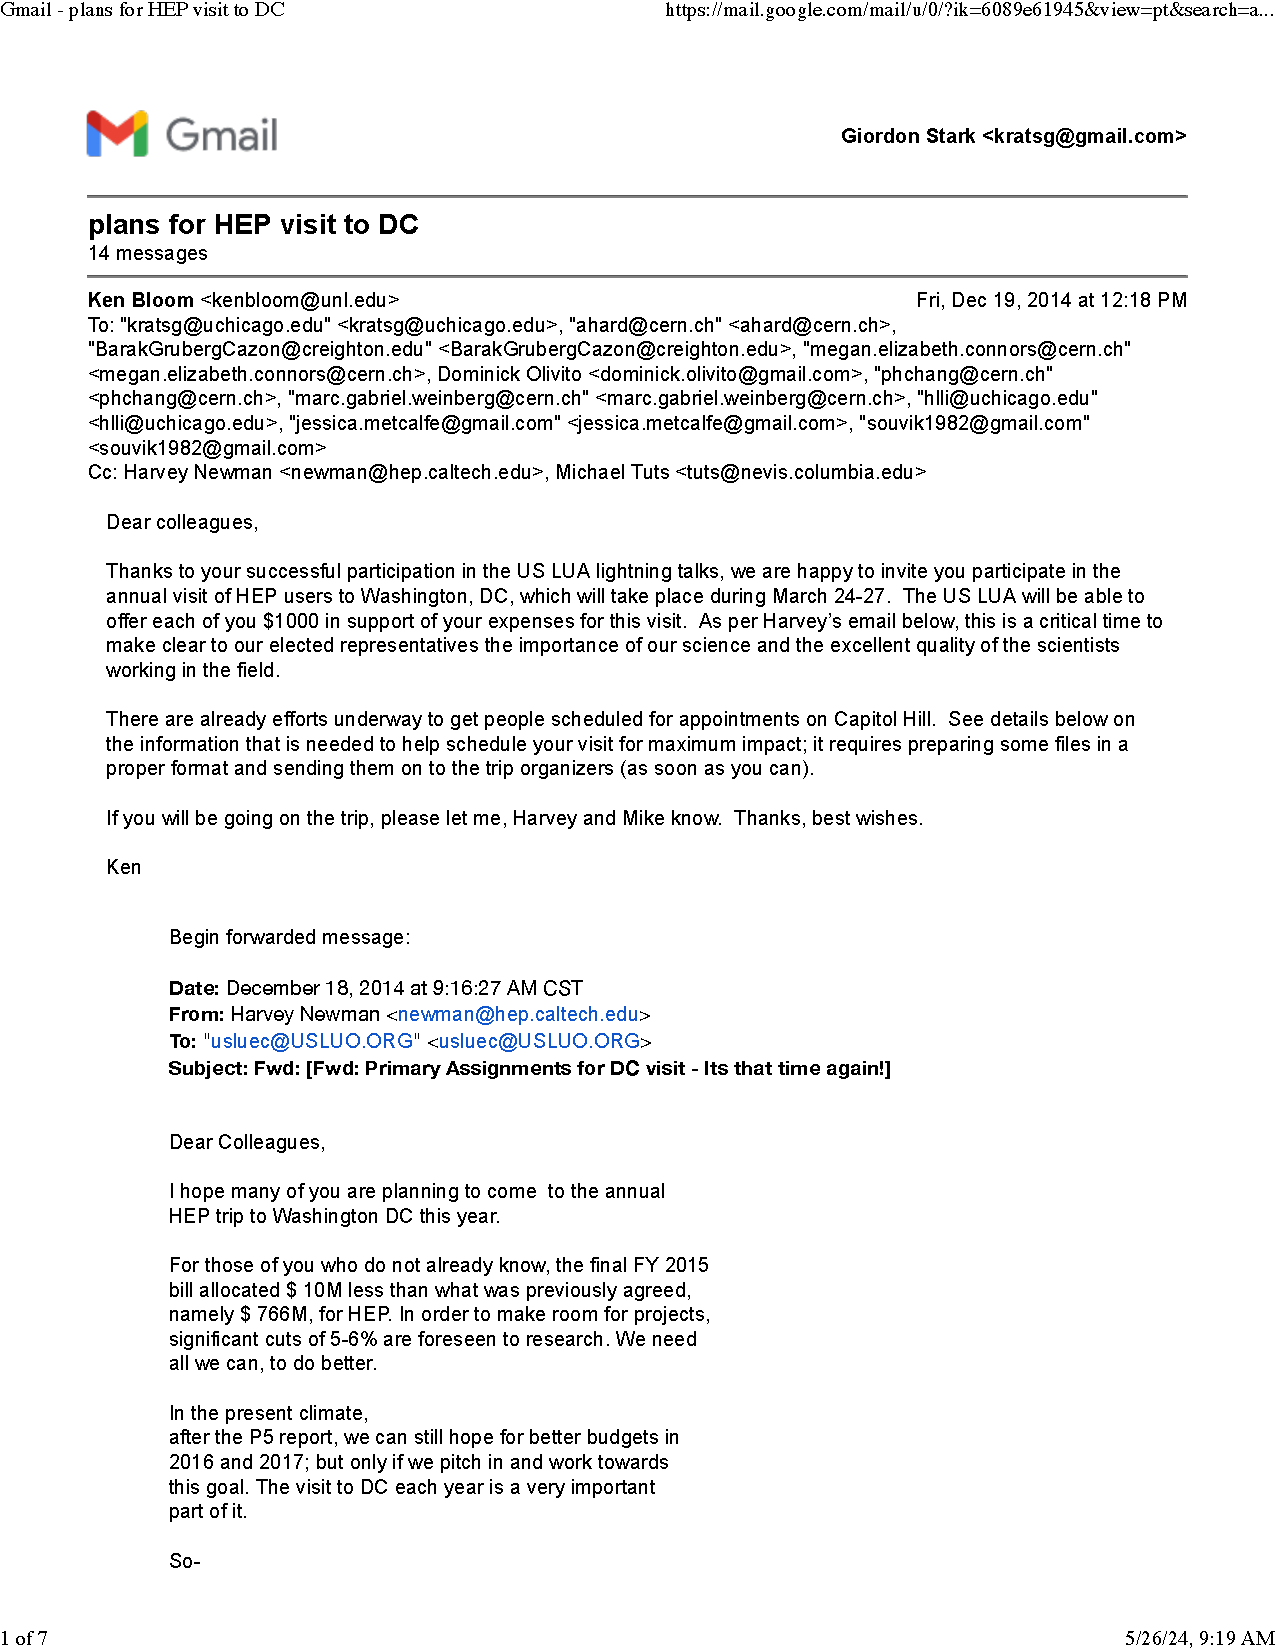
\includegraphics[width=0.9\textwidth]{attachments/D-research/usluaWinner}
\end{figure}

\begin{figure}[h!]
	\centering
	\caption{\textbf{Edward C. and Alice Stone Summer Undergraduate Research Fellow}: research fellowship. This is an email from the coordinator of the fellowship program. This fellowship supported my research on Submillimeter Wave Observatories.}
	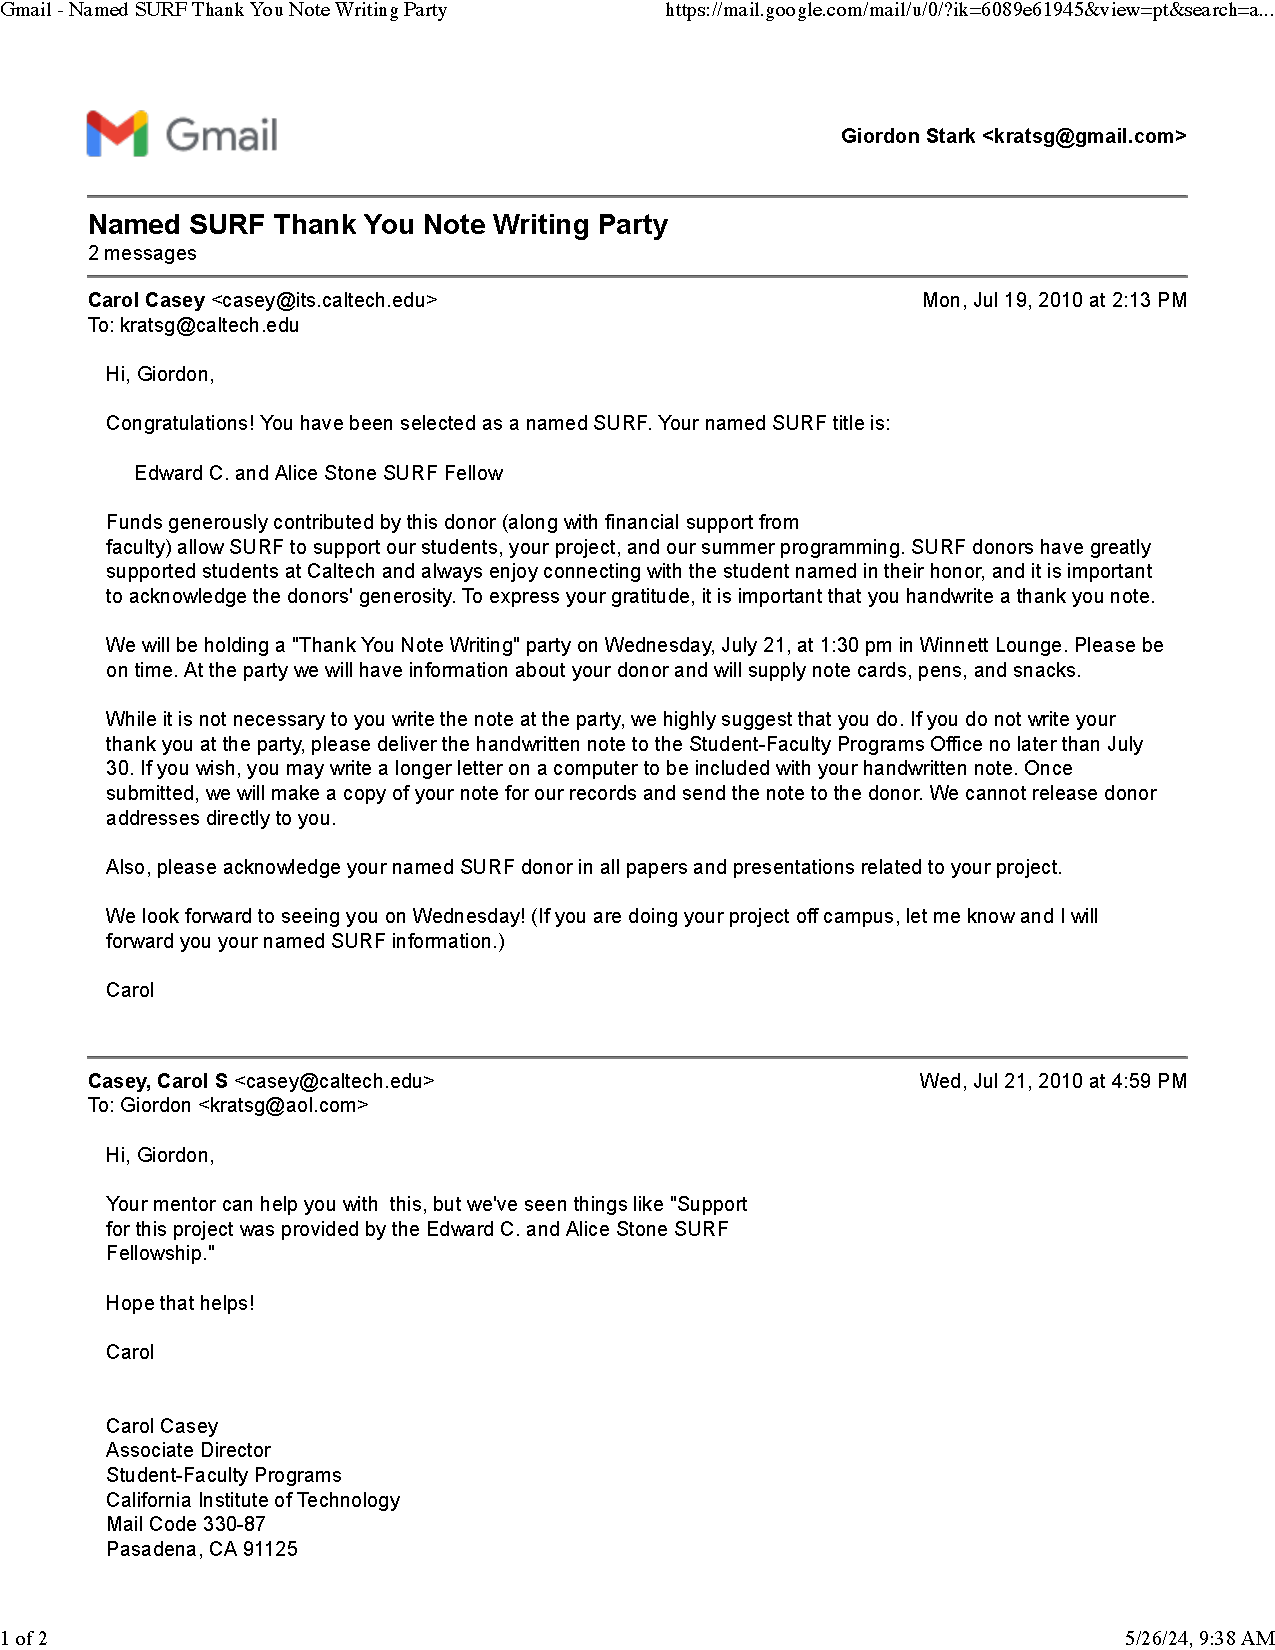
\includegraphics[width=0.9\textwidth]{attachments/D-research/SURFFellow}
\end{figure}


\chapter{Teaching qualifications portfolio}
% A total of 20 pages maximum of attachments to illustrate and document educational activities including for example
% a) Certificates of formal courses in teaching and learning in higher education
% b) Relevant Certificates of service
% c) Educational development plan, if applicable
% d) Processed course evaluation material (I have my student reviews)
I have scanned copies of written notes, as well as digital versions of various notes for discussion sections I led, as well as training notes for lab courses and classes I taught or led at Caltech and University of Chicago. In addition, there are training materials for workshops, bootcamps, and tutorials I organized / instructed for publicly available on the web (and continuously maintained / updated over time). There is a lot of material, and I am able to provide specific materials upon request. Below is a highlight / overview of the breadth.

\begin{itemize}
	\item UChicago TA Evaluations
	\item Example of notes for a discussion section
	\item Example ATLAS qualification project description
	\item Caltech Student Instructor Courses
	\item Caltech TA Award
\end{itemize}

\paragraph{Example ATLAS qualification projects description}
\begin{displayquote}
	{STUDENT} will develop a software package to perform statistical data
	analysis on data from ITk Pixel Module QC results for pre-production, with
	a focus on the electrical testing portions. This package will be developed
	in python, documented, and use Git version-control. GitLab at CERN will be
	used to host the package in the ITk Pixel Module group
	(https://gitlab.cern.ch/atlas-itk/pixel/module). The project will rely on
	existing work, itkdb (https://itkdb.docs.cern.ch/), for all interactions
	with the ATLAS ITk Production Database. The package will be a collection of
	different types of data analysis on the ITk Pixel Module QC results, each
	with its own configuration that can also be serialized using JSON. This
	configuration will have two parts described below. The first part is about
	the dataset of interest; describing which modules to include and which data
	linked to them to perform the analysis. The second part is about the
	processing of the datasets; describing the analysis to execute and
	registering the outputs to be saved. The deliverables of the software will
	be to analyse the distribution of a given QC measurement across modules of
	various origins and across multiple QC stages. It should also be able to
	investigate standard reporting such as the observed yield, e.g., by
	identifying the parameters of the quality control that have the strongest
	impact. The work will be documented both in the GitLab project as well as
	within an internal note. Regular progress reports will be made in the ATLAS
	ITk Pixel Module meetings.
\end{displayquote}
-- \textit{written for a Physics PhD student at Saclay CEA, with myself as technical supervisor}

\begin{displayquote}
	This technical project deals with the development and implementation of QA/QC
	procedures for the ATLAS ITk Pixel On-Detector Services. All of the
	institutes working with Type-1 electrical services have acquired Cirris
	cable tester units, but these units do not have the software interface
	needed for testing or uploading results to the ITk production databases.
	The deliverable for this project is the common software framework and
	standard operating procedures needed to integrate the Cirris cable testers
	into the ITk pixel QA/QC workflow. The project comprises the following 3
	main components: 1. Test definition. In collaboration with the Type-1
	institutions, develop the test definition, including Cirris configuration
	files, pin mapping definitions, and translation to Cirris language (Lua
	programming language). 2. Output parsing/transformation. Parse raw output
	to prepare summary tables for operators, perhaps even a graphical
	representation/mapping for easier interpretation and for documentation. 3.
	Interface with global production database. Working with Type-1 and database
	experts, preparing the JSON file, checking results graphically (see \#2
	above), and using ITkDB interface to upload the results to the production
	database. At the moment, the local DB for the services is not uniformly
	defined, so the task focuses on the global production DB instead. The
	progress on this task will be monitored in the ITk Pixel Electronics
	meeting and the Production Database meetings. It will be summarized at the
	end in an ATLAS note.
\end{displayquote}
-- \textit{written for a Physics PhD student at UCSC, with myself as local supervisor}


\section{Certificates of formal courses in teaching and learning in higher education \noneyet} \label{sec:certificates-of-formal-courses-in-teaching-and-learning-in-higher-education-noneyet}
\section{Relevant Certificates of service \noneyet} \label{sec:relevant-certificates-of-service-noneyet}
\section{Educational development plan, if applicable \normalsize{\textit{-- not applicable}}} \label{sec:educational-development-plan-if-applicable-not-applicable}
\section{Course evaluations} \label{sec:course-evaluations}

\section{Portfolio of leadership and administration} \label{sec:portfolio-of-leadership-and-administration}
% Formal leadership courses and certificates of service

\setcounter{chapter}{6}
\chapter{Portfolio of cooperation with wider society, innovation, and entrepreneurship}
% A total of 10 pages maximum of selected attachments may be included to illustrate and document the activities
\begin{itemize}
	\item ASLCore screenshot
	\item Red Cross Award
	\item Media on my website
	\item Dissertation defense Game of Thrones advertisement
\end{itemize}

\end{document}
